\subsubsection{Parasitäre Paramter}\label{subsec:parasitparam}
In diesem Unterkapitel werden grundsätzlich die Einflüsse und Eigenschaften von Parasitären Paramentern in Realen Bauteilen, besonders Spule und Kondensator, erklärt

Hierbei müssen die elektrischen Bauelemente, wie Spule und Kondensator mit den passenden parasitären Parameter ergänz werden. In Abbildung \ref{fig:stray_L} und \ref{fig:stray_C} werden die parasitären Parameter von Spule und Kondensator gezeigt.
\begin{figure}[H]
	\begin{minipage}[h]{0.45\linewidth}
		\centering
		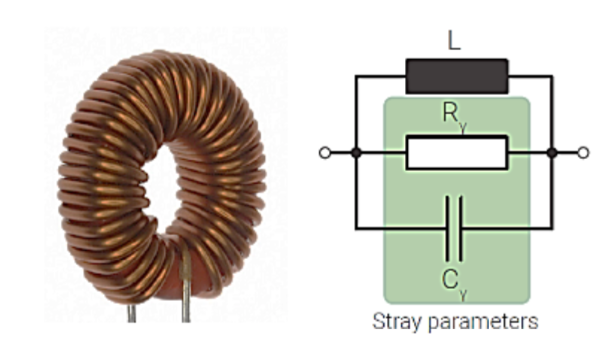
\includegraphics[width = 5cm]{stray_L.png}
		\label{fig:stray_L}
		\caption{Parasiäre Elemente einer Induktivität \cite{aufgabenstellung}}
	\end{minipage}
	\begin{minipage}[h]{0.45\linewidth}
		\centering
		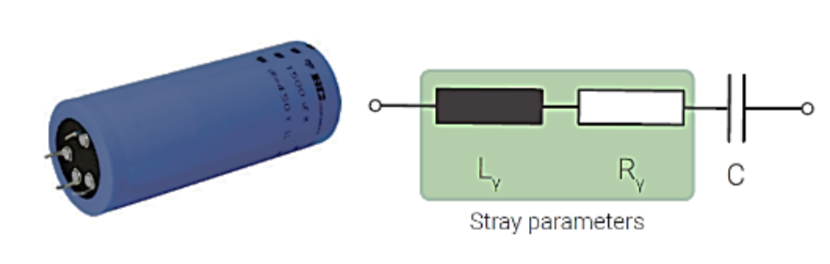
\includegraphics[width = 7cm]{stray_C.png}
		\label{fig:stray_C}
		\caption{Parasiäre Elemente einer Kapazität \cite{aufgabenstellung}}
	\end{minipage}
\end{figure}